\chapter{Análise do Problema} \label{cap:analise}

Tal como apresentado anteriormente, este projeto consiste na realização do sistema informático que designamos por Water Watcher, constituído essencialmente por duas partes: a interface para os utilizadores e o elemento servidor. Estes irão interagir com o local onde estão armazenados os dados, local este que pode ser entendido de forma genérica como uma base de dados, e com o sistema informático que a empresa de sistema de fornecimento de água já possui e utiliza.\\
A componente de interação com o utilizador terá como função principal a “leitura” do contador, ou seja, através da câmara do dispositivo, é capturada uma imagem da contagem medida pelo aparelho contador de consumo de água. Este elemento terá garantias de robustez em cenários de utilização real, isto é, deverá saber lidar de forma correta com situações anómalas como o mau estado dos contadores ou leituras erradas por erro do sistema ou do cliente.\\
Leituras erradas deverão, de forma geral, ser substituídas pela estimativa já calculada pela empresa, ou por uma nova estimativa calculada por este sistema informático.\\
Este componente poderá também apresentar informações relativas ao consumo de água como estatísticas de consumo em intervalos de tempo definidos, aviso de gastos menores/maiores que o esperado e outras possíveis informações pertinentes ao cliente sobre este serviço.\\
Outro elemento deste sistema informático será um servidor, cuja função é, resumidamente, interpretar os caracteres das imagens captadas pelos utilizadores e mediar a comunicação entre a interface dos utilizadores e o local onde estão armazenados os dados. Também será o servidor o responsável por garantir a segurança deste sistema: assegurar a integridade das comunicações e garantir o correto acesso das várias funcionalidades do sistema apenas aos utilizadores autorizados.\\
A figura \ref{fig:modelo} representa o sistema e os seus componentes. O servidor e a interface do utilizador são componentes intrínsecos do sistema, pelo que o sistema não existiria sem eles, enquanto que o sistema de gestão de base de dados será um componente do sistema porém independente. O sistema de gestão de consumos é um outro sistema com o qual o nosso vai comunicar.

\vspace{1cm} %espaço

\begin{figure}[ht!]
\centering
\resizebox{150mm}{!}{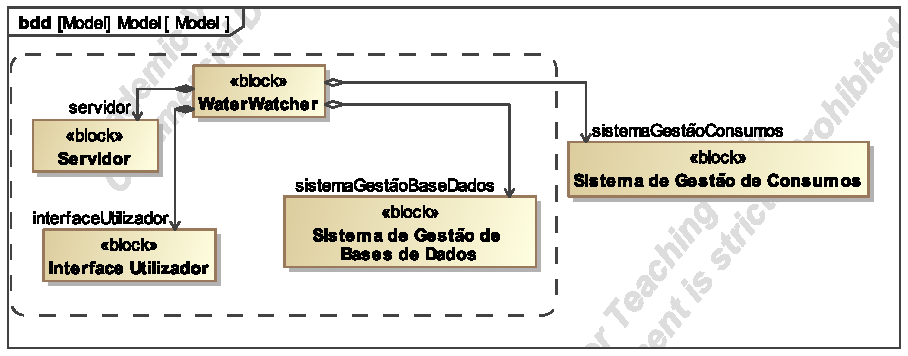
\includegraphics{diagramas/svg/bdd__Model.pdf}}
\caption{Arquitetura do sistema.}
\label{fig:modelo}
\end{figure}

Neste capítulo, na secção \ref{sec:req_sis} vamos explorar os requisitos que o sistema deve cumprir e na secção \ref{sec:casos_uso} os vários casos em que o sistema vai ser utilizado.

% REQUISITOS DO SISTEMA
\section{Requisitos do Sistema} \label{sec:req_sis}
Uma das primeiras etapas no desenvolvimento de um sistema informático deve ser o levantamento dos requisitos do sistema, ou seja, averiguar as várias funcionalidades que o sistema deverá ter para que este resolva os problemas que se propõe a resolver.\\
Os requisitos classificam-se como funcionais ou não funcionais. Os requisitos funcionais são requisitos que o sistema tem obrigatoriamente que cumprir para operar corretamente. Os requisitos não funcionais são características que, apesar de não serem essenciais ao funcionamento do sistema, garantem funcionalidades importantes para conferir qualidade de utilização, segurança e um bom desempenho do sistema.

% REQUISITOS DA INTERFACE UTILIZADOR
\subsection{Requisitos da Interface com o Utilizador.}
A interface de utilizador vai-se dividir em duas interfaces. Uma interface que será comum aos utilizadores e aos administradores e uma interface específica aos administradores, para que haja uma correta separação de funções e permissões no sistema. 

\subsubsection{Interação com o Utilizador}
O sistema terá uma interface de utilização para que os utilizadores possam fácil e intuitivamente efetuar as diversas operações que o sistema disponibiliza. Os vários requisitos estão descritos na tabela \ref{tab:req_utilizador}.

%TABELA INTERACAO UTILIZADOR
\begin{center}
\begin{tabular}[c]{||p{1.5cm} | p{3cm} | p{6cm} | p{2.5cm}||} 
\hline
Requisito & Função & Descrição & Funcional/Não Funcional\\ %[0.5ex] 
\hline\hline
1 & Interação com o utilizador & Interfaces com as quais o utilizador possa interagir para efetuar diferentes operações. & Funcional\\ 
\hline
1.1 & Interação de leitura de contagem & Interface que permite ao utilizador efetuar a captura da imagem do contador para ser efetuada a leitura dos carateres. & Funcional\\
\hline
1.1.1 & Envio de leitura & Enviar a fotografia tirada pelo utilizador para outro elemento do sistema, respeitando os vários procedimentos para fazer um correto envio da imagem. & Funcional\\
\hline
1.2 & Interface de autenticação & 
Interface que permita que o utilizador se autentique. A autenticação divide-se em registo e {\textit{log in}}. & Funcional\\
\hline
1.3 & Interface de estatísticas & 
Interface dedicada a apresentar ao utilizador estatísticas relacionadas com o seu consumo de água. & Funcional\\ %[1ex] 
\hline
\end{tabular}
\captionof{table}{Requisitos da interface com o utilizador.} 
\label{tab:req_utilizador}
\end{center}

\subsubsection{Interação com o Administrador}
O sistema deverá ter na sua composição uma interface de utilização para os utilizadores administradores. Esta interface de utilização terá um papel de gestão dos dados dos clientes e outras funções como emitir alertas/notificações para todos ou alguns utilizadores.
Todo este módulo do sistema terá de apresentar várias garantias de segurança, nomeadamente, garantir a integridade das comunicações e a segurança dos dados. Os vários requisitos estão descritos na tabela \ref{tab:req_admin}.

%TABELA INTERACAO ADMIN
\begin{center}
\begin{tabular}[c]{||p{1.5cm} | p{3cm} | p{6cm} | p{2.5cm}||} 
\hline
Requisito & Função & Descrição & Funcional/Não Funcional\\ %[0.5ex] 
\hline\hline
2 & Interação com o administrador & Interface de utilização para os utilizadores administradores. & Funcional\\ 
\hline
2.1 & Gestão de dados & Interface que permita a utilizadores com papéis de administração inserir, modificar e apagar estes dados. & Funcional\\
\hline
2.2 & Anúncios & Poderá ainda ser necessário contactar um ou vários clientes em específico. & Não Funcional\\
\hline
\end{tabular}
\captionof{table}{Requisitos da interface com utilizadores com permissões de administrador.} 
\label{tab:req_admin}
\end{center}

% REQUISITOS DO SERVIDOR
\subsection{Requisitos do Servidor}
 
Será o servidor o módulo responsável neste sistema por interpretar os caracteres presentes nas imagens que os vários utilizadores capturam dos seus contadores.
O servidor será responsável por guardar persistentemente na base de dados as contagens de água relativas a cada utilizador.
Para interpretar os caracteres presentes nas fotografias dos contadores, o servidor terá de recorrer a um processo de OCR({\it{Optical Character Recognition}} ou Reconhecimento Óptico de caracteres).
Para além desta função, o servidor terá de cumprir os requisitos descritos na tabela \ref{tab:req_serv}.

%TABELA REQ SERVIDOR
\begin{center}
\begin{tabular}[c]{||p{1.5cm} | p{2.6cm} | p{6cm} | p{2.5cm}||} 
\hline
Requisito & Função & Descrição & Funcional/Não Funcional\\ %[0.5ex] 
\hline\hline
3 & Segurança & À semelhança da interface de utilização, o servidor terá também de garantir a integridade das comunicações e a segurança dos dados. & Não Funcional\\ 
\hline
3.1 & Opacidade dos dados & Os dados transportados nas comunicações entre os diversos sistemas não poderão ser visíveis para possíveis atacantes. & Não Funcional\\
\hline
3.2 & Integridade dos dados & Teremos que nos certificar que os dados que chegam ao servidor foram enviados de uma origem fidedigna e que os dados não foram alterados. & Não Funcional\\
\hline\hline
4 & Aceder à informação de utilizador & O servidor será capaz de aceder ao local onde estão armazenadas as informações dos utilizadores. & Funcional\\ 
\hline
4.1 & Editar a informação de utilizador &Por alterações relativas aos contadores, ao contrato ou às informações pessoais do utilizador, como uma nova morada, será importante ser possível que o servidor tenha, nesse caso, permissões para corrigir as informações guardadas relativas a um utilizador de forma a que esta fique coerente e correta. & Funcional\\
\hline
4.2 & Obter a informação de utilizador & Também será essencial obter informações sobre os vários utilizadores do serviço de forma a confirmar as suas credências de autenticação ou para apresentar informações personalizadas. & Funcional\\
\hline
\end{tabular}
\captionof{table}{Requisitos do servidor.} 
\label{tab:req_serv}
\end{center}


% CASOS DE USO
\section{Casos de Uso} \label{sec:casos_uso}
É importante averiguar qual a utilização que o sistema terá e como é que os utilizadores e outros sistemas interagem com o Water Watcher. Para além disso, dado que o sistema será composto por vários módulos, também devemos planear quais as interações entre eles. A figura \ref{fig:uso_sistema} apresenta de forma geral os casos de uso do sistema.

\begin{figure}[h!]
\begin{center}
\resizebox{130mm}{!}{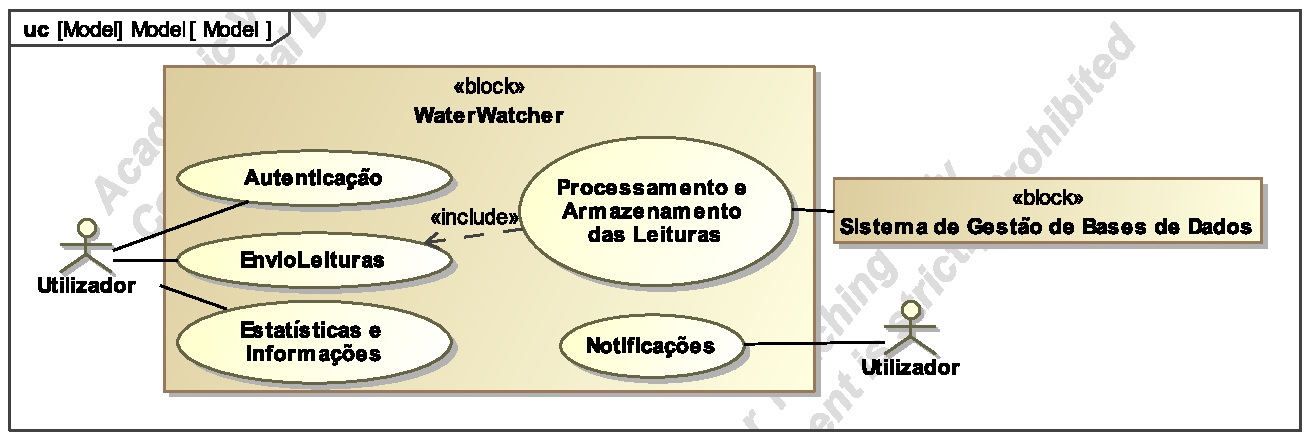
\includegraphics{diagramas/svg/uc__Model.pdf}}
\caption{Casos de uso do sistema.}
\label{fig:uso_sistema}
\end{center}
\end{figure}

Analisámos também os casos de uso específicos para cada componente do sistema, analisando as funções de cada um e as suas interações tanto com utilizadores como com outros componentes do sistema ou até outros sistemas.

% CASOS DE USO DO SERVIDOR
\subsection{Casos de Uso do Servidor}
O servidor está encarregado de receber as fotografias dos contadores enviadas pelos utilizadores e processá-las, ou seja, interpretar os caracteres na fotografia do contador para obter o resultado da contagem e enviar esse resultado para o sistema informático da empresa fornecedora de água.\\
Também é o responsável por mediar as interações das interfaces de utilização com a base de dados que contém a informação dos utilizadores, confirmando se o utilizador que fez o pedido pode ter acesso às informações que pede, efetuar o pedido à base de dados e enviar o resultado para o cliente que fez o pedido.\\
Qualquer mensagem recebida tem de ser avaliada para garantir a sua origem e garantir que o conteúdo não se alterou no processo da comunicação. As comunicações provenientes do servidor devem ser cifradas e assinadas de forma a que o destinatário saiba que foi, de facto, o servidor quem enviou essa mensagem e que o conteúdo da mensagem não sofreu alterações indevidas e também para que o conteúdo da mensagem não seja visível para alguém que tenha acesso indevido à mensagem durante o seu transporte.\\
Na figura \ref{fig:uso_serv1} estão presentes os casos de utilização em que o ator, ou seja, onde se iniciam as ações que promovem os processos no sistema, é a interface de utilizador, enquanto que na figura \ref{fig:uso_serv2} o ator é a empresa fornecedora ou a interface de utilização.

\vspace{3.5cm} %espaço

\begin{figure}[h!]
\begin{center}
\resizebox{130mm}{!}{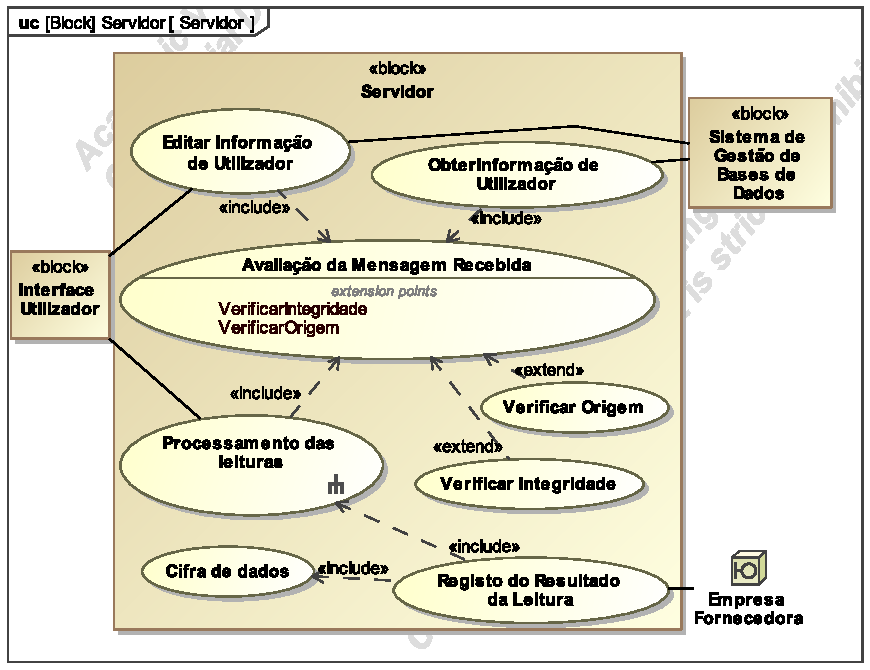
\includegraphics{diagramas/svg/uc__Servidor__Servidor.pdf}}
\caption{Casos de uso do servidor pela interface do utilizador.}
\label{fig:uso_serv1}
\end{center}
\end{figure}

\begin{figure}[h!]
\begin{center}
\resizebox{110mm}{!}{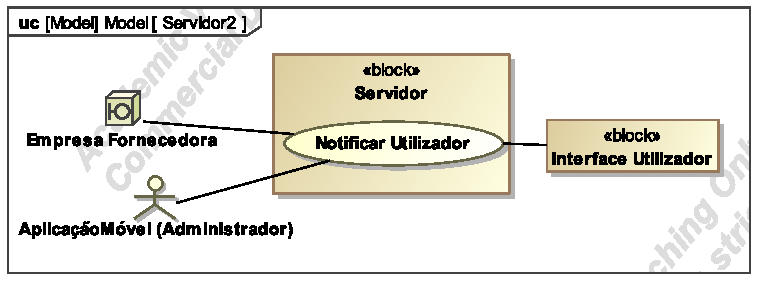
\includegraphics{diagramas/svg/uc__Servidor2.pdf}}
\caption{Casos de uso do servidor pela empresa fornecedora ou pelo administrador.}
\label{fig:uso_serv2}
\end{center}
\end{figure}

\vspace{1cm}%espaço

O processamento das leituras, como representado na figura \ref{fig:state_processamento} consiste inicialmente em verificar a origem e a integridade da mensagem recebida, descartando a mensagem caso o sistema detete que a mensagem não deva ser processada. Posteriormente é efetuado o reconhecimento dos caracteres na imagem e, caso o resultado deste processo apresente um valor válido para uma leitura, a contagem é registada para o utilizador que enviou a mensagem inicial.

\vspace{2cm}%espaço

\begin{figure}[h!]
\begin{center}
\resizebox{110mm}{!}{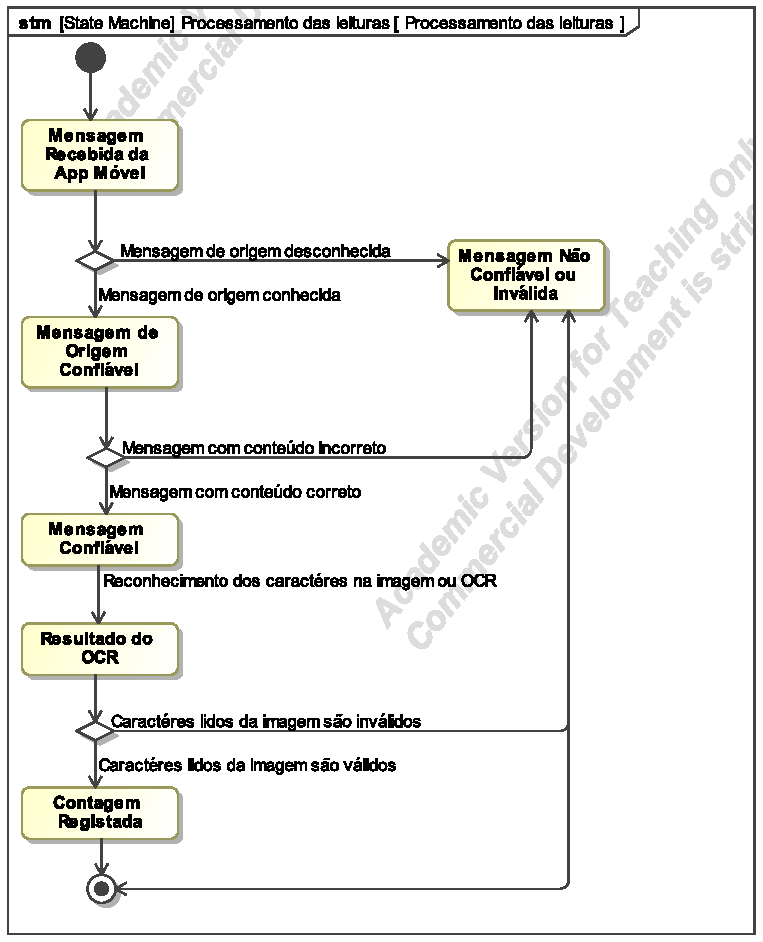
\includegraphics{diagramas/svg/stm__Processamento_das_leituras__Processamento_das_leituras.pdf}}
\caption{Processamento das leituras dos contadores.}
\label{fig:state_processamento}
\end{center}
\end{figure}


% CASOS DE USO DA APP MOVEL
\subsection{Casos de Uso da Interface de Utilização}
A interface de utilização é a parte do sistema que trata a interação com os utilizadores. É aqui que o utilizador se autentica, ou seja, efetua o seu registo quando utiliza o sistema pela primeira vez, sendo que nos próximos acessos será naturalmente apenas necessário o {\textit{log in}}.\\
Poderá posteriormente adicionar ou remover contadores e contratos, bem como alterar as suas informações pessoais. O utilizador pode ter acesso às suas estatísticas de consumo de água e a outras informações relativas ao serviço.\\
Também poderá então captar uma fotografia do contador para iniciar o processo de informar a empresa da sua contagem de água. À semelhança do servidor, as comunicações deverão ser cifradas e assinadas pelos mesmos motivos.\\
A figura \ref{fig:state_processamento} apresenta os casos de utilização da interface de utilização.

\vspace{1cm}%espaço

\begin{figure}[h!]
\begin{center}
\resizebox{140mm}{!}{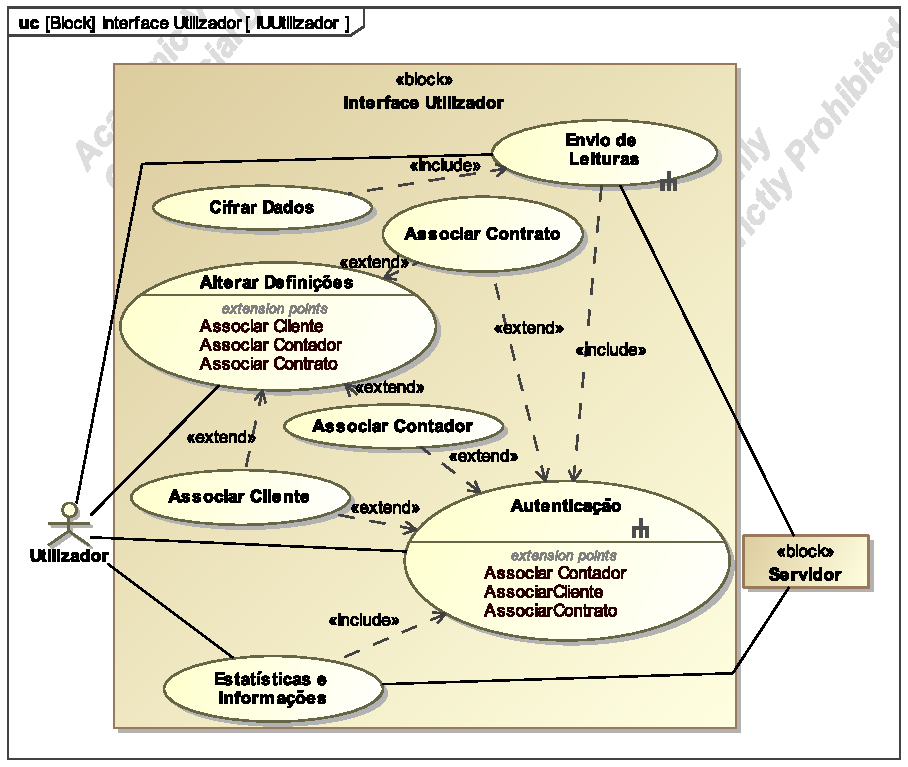
\includegraphics{diagramas/svg/uc__Interface_Utilizador__IUUtilizador.pdf}}
\caption{Casos de uso da interface de utilização.}
\label{fig:state_processamento}
\end{center}
\end{figure}

A autenticação, descrita na figura \ref{fig:state_autenticacao}, consiste em permitir ao utilizador criar uma conta nova ou aceder com as credenciais de uma conta já existente.

\begin{figure}[ht!]
\begin{center}
\resizebox{110mm}{!}{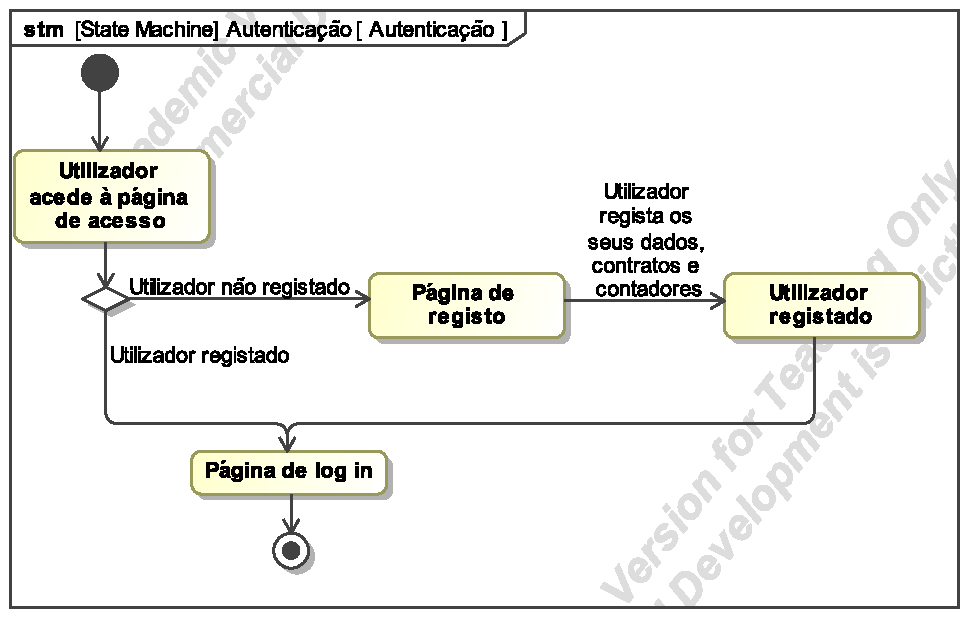
\includegraphics{diagramas/svg/stm__Autenticação__Autenticação.pdf}}
\caption{Processo de autenticação.}
\label{fig:state_autenticacao}
\end{center}
\end{figure}

A figura \ref{fig:state_envio} descreve o processo de envio de leituras, que começa com a ativação da câmara do dispositivo do utilizador de forma a que este possa captar uma fotografia do seu contador. Depois de tirada a fotografia, o sistema gera uma mensagem que contém esta fotografia, cifra e assina esta mensagem e envia-a para o servidor.

\begin{figure}[ht!]
\begin{center}
\resizebox{100mm}{!}{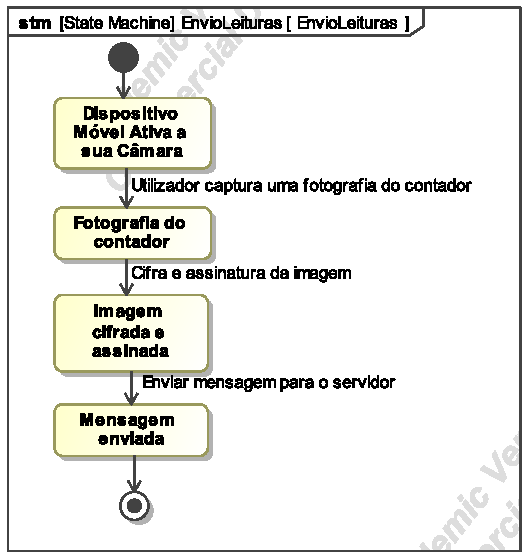
\includegraphics{diagramas/svg/stm__EnvioLeituras__EnvioLeituras.pdf}}
\caption{Processo de envio de leituras.}
\label{fig:state_envio}
\end{center}
\end{figure}












